\newpage
\section{Divide y Vencerás. Aplicaciones}
\begin{enumerate}[a)]
  \item \textbf{Geometría Computacional: }Construir la solución algorítmica (pseudocódigo) para la envolvente convexa (convex hull) de una nube de puntos en el plano, con la técnica Divide y Vencerás. Explicar claramente el desarrollo y calcular el tiempo de ejecución (Nota: debe ser O(n log n)).
  
  \textbf{Aproximación con fuerza bruta: }el metodo con fuerza bruta para determinar la convex hull consiste en construir una linea conectando dos puntos y entonces verificar si todos los puntos se encuentran en el mismo lado o no. De esta manera se tendran $n(n-1)/2$ lineas para n puntos, y cada linea se compara con los restantes $n-2$ puntos para ver si estos caen el mismo lado. Como resultado, la aproximacion con fuerza bruta require un tiempo $(O(n^3))$.

  \textbf{Aproximación con divide y vencerás: }Una solución mas eficiente a lo planteado en la aproximación con fuerza bruta es utilizando la estrategia algorítmica divide y vencerás planteando el siguiente algoritmo:
  \begin{itemize}
    \item Ordenar todos los puntos por sus coordenadas X, en caso de coincidir dos puntos con misma coordenada X entonces la coordenada Y se usara para desempatar
    \item Determinar los puntos de los extremos A y B, donde A representa el punto que se encuentra mas a la izquierda y B representa el punto que se encuentra mas a la derecha. A y B serian vertices de la convex hull. Se agregan lineas AB y BA al conjunto solucion
    \item Se busca un punto C que sera el mas alejado de la linea AB
    \item Se calcula la convex hull de los puntos a la izquierda y derecha de la linea AC. Luego se remueve la linea AB de la solucion original y se reemplaza por AC y CB
    \item Se procesan los puntos a la derecha de BA de la misma manera
    \item Encontrar la convex hull de los puntos a la izquierda y derecha de la linea que conecta los puntos mas lejanos de una convex hull especifica de manera recursiva
  \end{itemize}

\begin{lstlisting}[escapeinside={(*}{*)},style=java,caption= Algoritmo ConvexHull(P)]
 //P es un conjunto de puntos de entrada

 Ordenar todos los puntos en p y encontrar los dos puntos extremos A y B
 S1 (*$\leftarrow$*) conjunto de puntos a la derecha de la linea AB
 S2 (*$\leftarrow$*) conjunto de puntos a la derecha de BA
 Solucion (*$\leftarrow$*) AB seguido de BA

 Llamada FindHull(S1, A, B)
 Llamada FindHull(S1, B, A)
\end{lstlisting}

\begin{lstlisting}[escapeinside={(*}{*)},style=java,caption= Algoritmo FindHull(P)]
  if isEmpty(P) then
    return
  else
    C (*$\leftarrow$*) punto ortogonalmente mas alejado  de ambos
    Solucion (*$\leftarrow$*) reemplaza AB por AC seguido de CB
    Divide P - { C } en X0, X1 y X2

    Llamada FindHull(X1, A, C)
    Llamada FindHull(X2, C, B)
  end
 \end{lstlisting}

 \textbf{Ejemplo de ejecución: }

 \begin{figure}[!htb]
  \centering
  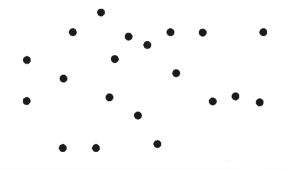
\includegraphics[width=7cm, scale=1]{Images/Punto3/ej1.png}
  \caption{Encontrar la convex hull para estos puntos}
\end{figure}

\textbf{Paso 1: }Se buscan los puntos mas a la izquierda y mas a la derecha del conjunto P y se los etiqueta como A y B. Se etiqueta el conjunto de puntos a la derecha de AB como $S_1$ y todos los puntos a la derecha de BA como $S_2$

\begin{figure}[!htb]
  \centering
  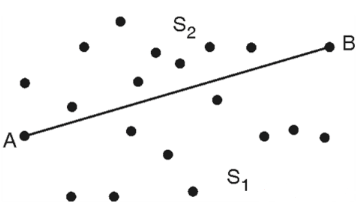
\includegraphics[width=7cm, scale=1]{Images/Punto3/ej2.png}
  \caption{}
\end{figure}

Solucion= $\{AB,BA\}$

Se hace una llamada recursiva a $FindHull(S_1, A, B)$ y $FindHull(S_2, B, A)$

\textbf{Paso 2: }$FindHull(S_1, A, B)$

Se busca el punto C ortogonalmente mas alejado de la linea AB

\begin{figure}[!htb]
  \centering
  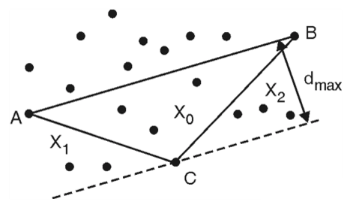
\includegraphics[width=7cm, scale=1]{Images/Punto3/ej3.png}
  \caption{}
\end{figure}

Solucion= $Solucion - \{AB\} \cup \{AB,BA\} = \{AC, CB, BA\}$

Se etiquetan las regiones $X_0$, $X_1$ y $X_2$ como se muestran en la Figura 4

Hace llamadas recursivas: $FindHull(X_1, A, C)$ y $FindHull(X_2, C, B)$

\textbf{Paso 3: }$FindHull(X_1, A, C)$

Se busca el punto D ortogonalmente mas alejado de la linea AC

\begin{figure}[!htb]
  \centering
  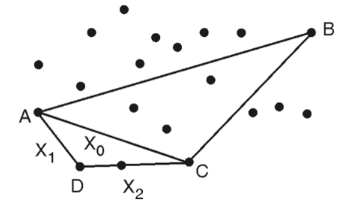
\includegraphics[width=7cm, scale=1]{Images/Punto3/ej4.png}
  \caption{}
\end{figure}

Solucion= $Solucion - \{AC\} \cup \{AD,DC\} = \{AD, DC, CB, BA\}$

Se etiquetan las regiones $X_0$, $X_1$ y $X_2$ como se muestran en la Figura 5

Hace llamadas recursivas: $FindHull(X_1, A, D)$ y $FindHull(X_2, D, C)$

Pero los conjuntos $X_1$ y $X_2$ están vacíos, por lo tanto el algoritmo retorna

\textbf{Paso 4: }$FindHull(X_2, C, B)$

Se busca el punto E ortogonalmente mas alejado de la linea CB

\begin{figure}[!htb]
  \centering
  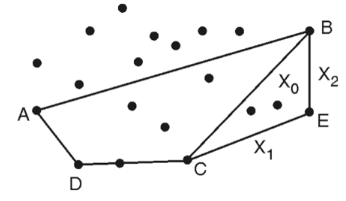
\includegraphics[width=7cm, scale=1]{Images/Punto3/ej5.png}
  \caption{}
\end{figure}

Solucion= $Solucion - \{CB\} \cup \{CE,EB\} = \{AD, DC, CE, EB, BA\}$

Se etiquetan las regiones $X_0$, $X_1$ y $X_2$ como se muestran en la Figura 6

Hace llamadas recursivas: $FindHull(X_1, C, E)$ y $FindHull(X_2, E, B)$

Pero los conjuntos $X_1$ y $X_2$ están vacíos, por lo tanto el algoritmo retorna, Ahora solamente restara explorar los puntos en $S_2$ a la derecha de la linea BA

\textbf{Paso 5: }$FindHull(S_2, B, A)$

Se busca el punto F ortogonalmente mas alejado de la linea BA

\begin{figure}[!htb]
  \centering
  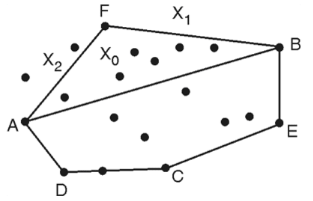
\includegraphics[width=7cm, scale=1]{Images/Punto3/ej6.png}
  \caption{}
\end{figure}

Solucion= $Solucion - \{BA\} \cup \{BF,FA\} = \{AD, DC, CE, EB, BF, FA\}$

Se etiquetan las regiones $X_0$, $X_1$ y $X_2$ como se muestran en la Figura 7

Hace llamadas recursivas: $FindHull(X_1, B, F)$ y $FindHull(X_2, F, A)$

Pero el conjunto $X_1$ esta vació, entonces la llamada $FindHull(X_1, B, F)$ retorna

\textbf{Paso 6: }$FindHull(X_2, F, A)$

Se busca el punto G ortogonalmente mas alejado de la linea FA

\begin{figure}[!htb]
  \centering
  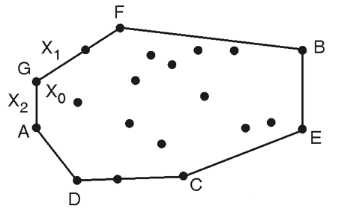
\includegraphics[width=7cm, scale=1]{Images/Punto3/ej7.png}
  \caption{}
\end{figure}

Solucion= $Solucion - \{FA\} \cup \{FG,GA\} = \{AD, DC, CE, EB, BF, FG, GA\}$

Se etiquetan las regiones $X_0$, $X_1$ y $X_2$ como se muestran en la Figura 8

Hace llamadas recursivas: $FindHull(X_1, F, G)$ y $FindHull(X_2, G, A)$

Pero los conjuntos $X_1$ y $X_2$ están vacíos, por lo tanto el algoritmo retorna, no quedan llamadas recursivas por lo que el poligono con aristas $\{AD, DC, CE, EB, BF, FG, GA\}$ es la convex hull de los puntos dados\\

\textbf{Análisis de eficiencia: }El paso de preprocesamiento consiste en ordenar los puntos de acuerdo a su coordenada X. El ordenamiento se puede realizar en un tiempo $O(nlog_2n)$. Encontrar los dos puntos mas elejados en la lista ordenada requiere un tiempo $O(1)$. Dividir los puntos en dos mitades $S_1$ y $S_2$ toma un tiempo $O(1)$ uniendo A y B. Generalmente $S_1$ y $S_2$ contiene la mitad de los puntos por lo tanto, computar recursivamente la convex hull de A y B tomara T(n/2) para cada uno. Fusionar las dos convex hulls se puede realizar en un tiempo lineal $O(n)$, encontrando el punto mas lejano ortogonalmente. Por lo tanto el tiempo de preprocesar los puntos estara dado por:

$T(n)=2T(n/2) + O(n) + O(1) = 2T(n/2)+ n \ldots (1)$

Resolviendo la recurrencia original para $n/2$

$T(n/2) = 2T(n/4) + n/2$

Sustistuyendo esto en ecuacion (1) se tiene

$T(n) = 2[2T(n/4) + n/2]+n= 2^2 T(n/2^2)+2n$


Luego de k sustituciones

$T(n) = 2^k T(n/2^k)+k\cdot n \ldots (2)$

La division del arreglo crea un arbol binario, cuya altura es $log_2n$, entonces se considerara que k crece hasta $log_2n$

$k = log_2n \rightarrow n=2^k$

Sustituyendo estos valores en la ecuacion (2)

$T(n) = n\cdot T(n/n)+log_2n\cdot n$

$\mathbf{T(n) = O(n\cdot log_2n)}$

  \item \textbf{Criptografía: }Construir la operación expoMod para calcular (1) y (2) a partir del esquema DyV de las diapositivas de teoría, y un programa que la utilice con las siguientes opciones:
  \begin{itemize}
    \item Generación de la clave pública.
    \item Carga del mensaje (digrafía) y cálculo de su representación en base 27.
    \item Generación del mensaje encriptado (cálculo del número y su representación en base 27)
    \item Descifrado del mensaje recepcionado.
  \end{itemize}
\end{enumerate}


\begin{lstlisting}[style=java,caption= Karatsuba (Algoritmo de multiplicacion de numeros grandes)]
  public class Karatsuba {
  public long mult(long num1, long num2) {
    // Si los numeros son lo suficientemente chicos los multiplica y retorna
    if (num1 < 10 && num2 < 10) {
      return num1 * num2;
    }

    // Obtiene longitudes de num1 y num2
    int num1Length = numLength(num1);
    int num2Length = numLength(num2);

    // Obtiene la longitud maxima entre ambos
    int maxNumLength = Math.max(num1Length, num2Length);

    // Obtiene la mitad de la longitud del num maxim (redondeando para arriba) n/2
    int halfMaxNumLength = (int) Math.ceil(maxNumLength / 2);

    // 10^(n/2) siendo n la cantidad de dugitos y n/2 = halfMaxNumLength
    long halfMaxNumLengthPowTen = (long) Math.pow(10, halfMaxNumLength);

    // Divide los numeros en mitades
    long x = num1 / halfMaxNumLengthPowTen;
    long y = num1 % halfMaxNumLengthPowTen;
    long w = num2 / halfMaxNumLengthPowTen;
    long z = num2 % halfMaxNumLengthPowTen;

    // Calcula los factores de la operaciun de manera recursiva
    long xw = mult(x, w);
    long xz = mult(x, z);
    long wy = mult(w, y);
    long yz = mult(y, z);

    return (xw * (long) Math.pow(10, halfMaxNumLength * 2) +
            ((xz + wy) * (long) Math.pow(10, halfMaxNumLength) + yz));

  }

  // Calcula la cantidad de digitos
  public int numLength(long n) {
    return ((int) (Math.log10(n)+1));
  }
}
\end{lstlisting}

\begin{lstlisting}[style=java,caption=Algoritmo de exponenciacion utilizando divide y venceras]
  public class ExpoDyV {
  public long expo(long  a, long n){
    if(n == 1) return a;

    long b;
    Karatsuba karatsuba = new Karatsuba();
    if(n%2==0){//Si n par
      b = expo(a,n/2);
      return karatsuba.mult(b, b);
    }else{
      return karatsuba.mult(a, expo(a, n-1));
    }
  }
}
\end{lstlisting}

\begin{lstlisting}[style=java,caption= Algoritmo de aritmetica modular con divide y venceras]
  public class ExpoMod {
  public long exponent(long a, long n, long z) {
    Karatsuba karatsuba = new Karatsuba();
    // Casos base
    if (a == 0) return 0;
    if (n == 0) return 1;

    // Si n par
    long y;
    if (n % 2 == 0)
    {
      y = exponent(a, n / 2, z); //Reduce el n a la mitad y hace llamado recursivo
      y = (karatsuba.mult(y, y)) % z;
    } else {//Si n impar
      y = a % z;
      y = (karatsuba.mult(y, exponent(a, n - 1, z) % z) % z);
    }
    return (long)((y + z) % z);
  }
}
\end{lstlisting}

\begin{lstlisting}[style=java,caption= Metodo main (Clase criptografia) ]
  static char [] tablaEquiNum = {'&','A','B','C','D','E','F','G','H','I','J','K','L','M','N','a','O',
        'P','Q','R','S','T','U','V','W','X','Y','Z'};
  public static void main(String[] args) {
    long p=17, q=43;
    Karatsuba obj = new Karatsuba();
    long publicKey= obj.mult(p,q);
    System.out.println("DATOS PUBLICOS");
    System.out.println("publicKey: "+publicKey);

    //Calcula thetaN
    long thetaN= (p-1)*(q-1);
    long e=getE(publicKey,thetaN);//e tiene que cumplir 1<e<thetaN ^ coprimo con N (pk) y thetaN
    System.out.println("e: "+e);


    //PARTE DE BERNARDO:

    System.out.println("\nBERNARDO ENCRIPTA");
    String w= encryptMessage("SI",e, publicKey);
    System.out.println("Mensaje encriptado w: "+w);


    //PARTE DE ALICIA:
    System.out.println("\nALICIA DESENCRIPTA");
    int w1= charToNumber(w.charAt(0));
    int w2= charToNumber(w.charAt(1));

    int numericValueW= w1*27+w2;
    System.out.println("Mensaje desencriptado: "+decryptMessage(e,thetaN,numericValueW,publicKey));
  }

\end{lstlisting}

\begin{lstlisting}[style=java,caption= Metodo encryptMessage ]
  public static String encryptMessage(String message, long e, long pk){ //El mensaje se sabe de 2 caracteres
  ExpoMod expoMod = new ExpoMod();
  //Obtiene numero base 27 de los caracteres de la cadena
  int x1 = charToNumber(message.charAt(0)); //Convierte letra a numero segun la tabla
  int x2 = charToNumber(message.charAt(1));

  int textNumber= x1 * 27 + x2;//Convierte el texto a base 27
  long y = expoMod.exponent(textNumber, e, pk); //encripta todo modificar 101 por e
  System.out.println("y: "+y);

  int y2=  (int)y%27;//y = x * 27 + z --> calcula z
  int y1= ((int)y-y2) /27;//x * 27 + z --> calcula x
  return ""+ tablaEquiNum[y1]+tablaEquiNum[y2];//Mensaje encriptado pasado a texto
}

\end{lstlisting}

\begin{lstlisting}[style=java,caption= Metodo decryptMessage ]
  public static String decryptMessage(long e, long thetaN, long y, long z){
    long d = getD(e,thetaN);
    System.out.println("d: "+d);
    ExpoMod expoMod = new ExpoMod();
    long decryptNumber = expoMod.exponent(y,d,z);
    int secondCaract=  (int)decryptNumber%27;//y = x * 27 + z --> calcula z
    int firstCaract= ((int)decryptNumber-secondCaract) /27;//x * 27 + z --> calcula x
    return ""+ tablaEquiNum[firstCaract]+tablaEquiNum[secondCaract];//Mensaje encriptado pasado a texto
  }

\end{lstlisting}

\begin{lstlisting}[style=java,caption= Metodo getE ]
  public static long getE(long N, long thetaN){
    boolean finded=false;
    int e=2;
    while(!finded && e < thetaN){ //Primer condicion
      if(checkCoprimes(e,N) && checkCoprimes(e,thetaN)){
        finded=true;
      }else{
        e++;
      }
    }
    if(!finded){//Si no encuentra devuelve -1
      e=-1;
    }
    return e;
  }

\end{lstlisting}

\begin{lstlisting}[style=java,caption= Metodo getD ]
  public static long getD(long e, long thetaN){ 
  long d= 1;
  while(((e * d)%thetaN)!=1 ){
    d++;
  }
  return d;
}

\end{lstlisting}

\begin{lstlisting}[style=java,caption= Metodo checkCoprimes]
  public static boolean checkCoprimes(long a,long b){
    boolean coprimes=false;
    if(checkCoprimesAux(a,b)==1){
      return true;
    }
    return coprimes;
  }
  public static long checkCoprimesAux(long a, long b){
    if (a == 0 || b == 0)
      return 0;

    // base case
    if (a == b)
      return a;

    // a is greater
    if (a > b)
      return checkCoprimesAux(a-b, b);

    return checkCoprimesAux(a, b-a);
  }

\end{lstlisting}

\begin{lstlisting}[style=java,caption= Metodo charToNumber ]
  public static int charToNumber(char character){//Base 26 (sin enie (a latex no le gusta la letra)) arrancando en 1
    return new String(tablaEquiNum).indexOf(character);
  }

\end{lstlisting}

\begin{figure}[!htb]
  \centering
  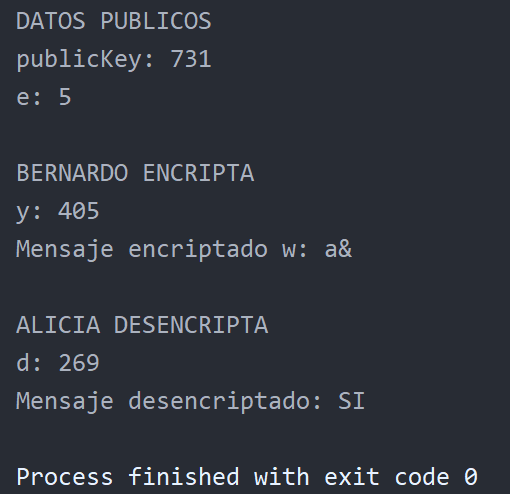
\includegraphics[width=7cm, scale=1]{Images/Punto3/SalidaConsolaCrypto.png}
  \caption{Salida por consola al encriptar y desencintar el mensaje ``SI''}
\end{figure}